\usetikzlibrary{calc,arrows.meta}
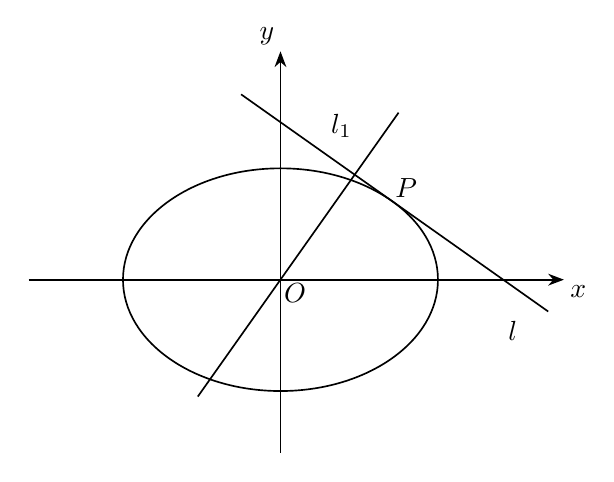
\begin{tikzpicture}[x=1cm,y=1cm,line width=.6pt,font=\normalsize,>=Stealth]
\coordinate (O) at (0,0);
\coordinate (P) at (1.4142,1);
\draw[->] (-3.2,0)--(3.6,0) node[anchor=north west,inner sep=0pt,xshift=2pt,yshift=-2pt] {$x$};
\draw[->] (0,-2.2)--(0,2.9) node[anchor=south east,inner sep=0pt,xshift=-2pt,yshift=2pt] {$y$};
\draw (O) ellipse[x radius=2cm,y radius=1.4142cm];
\draw (-1.05,-1.4849)--(1.5,2.1213);
\draw (-0.5,2.3536)--(3.4,-0.4041);
\node[below right,inner sep=1pt] at (O) {$O$};
\node[above right,inner sep=1pt] at (P) {$P$};
\node[left,inner sep=1pt] at (0.95,1.95) {$l_1$};
\node[right,inner sep=1pt] at (2.85,-0.65) {$l$};
\end{tikzpicture}
